\documentclass[10pt]{article}
\usepackage[english]{babel}
\usepackage{../../../meta-inf/lib/naproche}
\usepackage{amssymb}
\usepackage{mathtools} % for \coloneq

\usepackage{stex-highlighting}
\providebool{emph} % "\newbool{emph}" does not work...
\setbool{emph}{false}
\colorlet{emphcolor}{violet}
\let\oldemph\emph
\renewcommand\emph[1]{\setbool{emph}{true}\ifbool{forthel}{\textcolor{emphcolor}{\itshape#1}}{\oldemph{#1}}\setbool{emph}{false}}
\renewcommand{\varemph}[1]{\ifbool{emph}{\textcolor{emphcolor}{#1}}{\textcolor{black}{#1}}}

\usepackage[right=6cm,left=3cm,bottom=3cm,marginparwidth=5cm]{geometry}

\usepackage{fancyhdr}
\renewcommand{\sectionmark}[1]{\markboth{#1}{}} 
\def\libarchive{}
\pagestyle{fancy}
\fancyhead[L]{\libarchive}
\fancyhead[C]{\nouppercase\leftmark}  % section title
\fancyhead[R]{\thepage}               % page number
\fancyfoot[C]{}                       % No page number in footer

\usepackage[nobottomtitles]{titlesec}
\titlespacing*{\section}{0pt}{30pt}{0pt}
\titlespacing*{\subsection}{0pt}{30pt}{0pt}
\titlespacing*{\subsubsection}{0pt}{30pt}{0pt}

\documentclass[12pt,oneside]{book}

\usepackage[foundations]{../../lib/tex/naproche}
\usepackage{../../lib/tex/libraries}
\usepackage{graphicx}
\usepackage{float}
\usepackage{caption}
\usepackage{footnote}

\makesavenoteenv{tabular} % Make footnotes work in tabular environments


\title{Foundations of Mathematics}
\author{Marcel Schütz}
\date{2022}

\begin{document}
  \maketitle

  \tableofcontents

  \begin{figure}[H]
    \centering
    \fbox{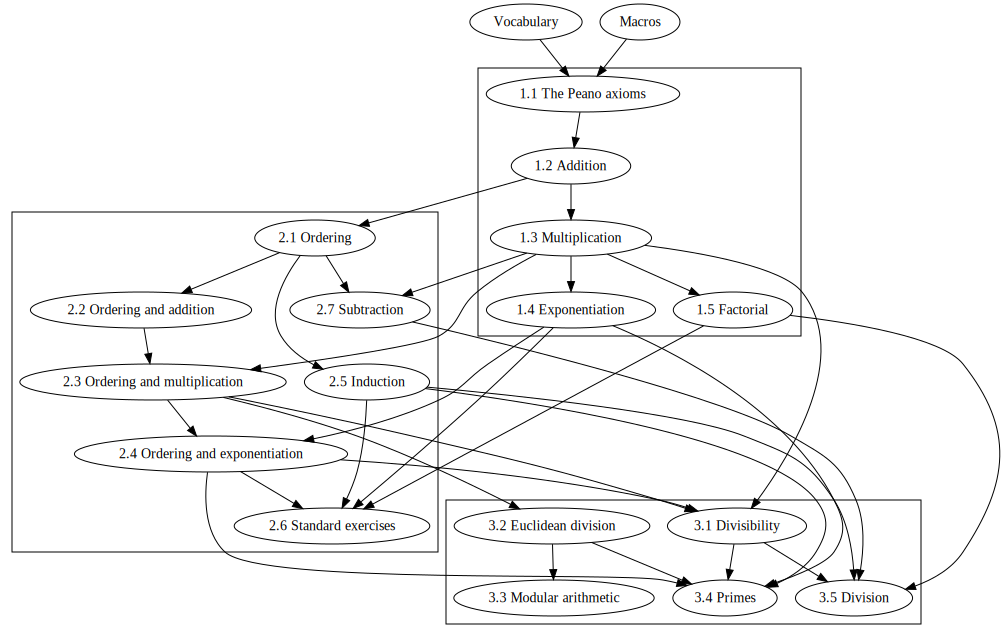
\includegraphics[width=0.9\linewidth]{./dependency-graph/graph.png}}
    \caption*{Interdependencies of the chapters}
  \end{figure}


  \section*{Introduction}

  This is a library providing a foundation of mathematics based on a
  Kelley-Morse like class theory with urelements.
  It introduces common operations on classes like unions or intersections
  (\cref{chapter:classes}) together with detailed proofs of their algebraic
  properties (\cref{chapter:computation-laws-for-classes}), the symmetric
  difference of two classes (\cref{chapter:symmetric-difference}) and the
  notions of ordered pairs and Cartesian products
  (\cref{chapter:pairs-and-products}) as well as proofs of the algebraic
  properties of the latter (\cref{chapter:computation-laws-for-products}).
  Moreover, it provides common operations on maps (\cref{chapter:maps}), various
  properties of images and preimages (\cref{chapter:image-and-preimage}) and the
  notions of injectivity, surjectivity, bijectivity
  (\cref{chapter:injections-surjections-bijections}) and invertibility of maps
  (\cref{chapter:invertible-maps}).
  The library provides an axiom system characterizing sets (\cref{chapter:sets})
  and, furthermore, it covers the notions of binary relations
  (\cref{chapter:binary-relations}), fixed-points of subset preserving maps
  (\cref{chapter:fixed-points}), including and equinumerosity
  (\cref{chapter:equinumerosity}).

  As two famous results it includes the Knaster-Tarski fixed point theorem
  (\cref{FOUNDATIONS_12_8420450166112256}) and the Cantor-Schröder-Bernstein
  theorem (\cref{FOUNDATIONS_13_1913663275401216}).

  \paragraph*{Usage.}
  At the very beginning of each chapter you can find the name of its source
  file, e.g. \path{foundations/sections/01_classes.ftl.tex} for
  \cref{chapter:classes}. This filename can be used to import the chapter via
  \Naproche's \texttt{readtex} instruction to another ForTheL text, e.g.:
  \begin{center}
    \verb`[readtex \path{foundations/sections/01_classes.ftl.tex}]`
  \end{center}

  \paragraph*{Checking times.}
  The checking times for each of the chapters may vary from computer to
  computer, but on mid-range hardware they are likely to be similar to those
  given in table below:

  \begin{center}
    \begin{tabular}{c|c|c}

      & \multicolumn{2}{c}{\textbf{Checking time}}
      \\
      \textbf{Chapter}
      & \textbf{without dependencies}     & \textbf{with dependencies}
      \\ \hline
      \ref{chapter:classes}
      & 00:04 min                         & 00:04 min
      \\
      \ref{chapter:computation-laws-for-classes}
      & 00:12 min                         & 00:16 min
      \\
      \ref{chapter:symmetric-difference}
      & 00:32 min                         & 00:48 min
      \\
      \ref{chapter:pairs-and-products}
      & 00:08 min                         & 00:12 min
      \\
      \ref{chapter:computation-laws-for-products}
      & 01:36 min                         & 01:56 min
      \\
      \ref{chapter:maps}
      & 01:13 min                         & 01:25 min
      \\
      \ref{chapter:image-and-preimage}
      & 01:28 min                         & 02:53 min
      \\
      \ref{chapter:injections-surjections-bijections}
      & 00:38 min                         & 02:03 min
      \\
      \ref{chapter:invertible-maps}
      & 02:20 min                         & 04:23 min
      \\
      \ref{chapter:sets}
      & 02:17 min                         & 06:40 min
      \\
      \ref{chapter:binary-relations}
      & 00:14 min                         & 06:54 min
      \\
      \ref{chapter:fixed-points}
      & 00:33 min                         & 07:13 min
      \\
      \ref{chapter:equinumerosity}
      & 01:48 min                         & 09:01 min
    \end{tabular}
  \end{center}


  \subfile{sections/01_classes.ftl.tex}
  \subfile{sections/02_computation-laws-for-classes.ftl.tex}
  \subfile{sections/03_symmetric-difference.ftl.tex}
  \subfile{sections/04_pairs-and-products.ftl.tex}
  \subfile{sections/05_computation-laws-for-products.ftl.tex}
  \subfile{sections/06_maps.ftl.tex}
  \subfile{sections/07_image-and-preimage.ftl.tex}
  \subfile{sections/08_injections-surjections-bijections.ftl.tex}
  \subfile{sections/09_invertible-maps.ftl.tex}
  \subfile{sections/10_sets.ftl.tex}
  \subfile{sections/11_binary-relations.ftl.tex}
  \subfile{sections/12_fixed-points.ftl.tex}
  \subfile{sections/13_equinumerosity.ftl.tex}
\end{document}

\begin{document}
  \begin{imports}
    \begin{forthel}
      %[prove off][check off]
      [readtex \path{libraries/source/foundations/classes.ftl.tex}]
      %[prove on][check on]
    \end{forthel}
  \end{imports}


  \section*{Ordered Pairs and Cartesian Products}

  \subsection*{Pairs}

  \begin{forthel}
    \begin{axiom}[id=FOUNDATIONS_04_8464577431863296,printid]
      Let $a, a', b, b'$ be objects.
      If $(a, b) = (a', b')$ then $a = a'$ and $b = b'$.
    \end{axiom}
  \end{forthel}

  \begin{forthel}
    \begin{definition}[id=FOUNDATIONS_04_4782386822774784,printid]
      A pair is an object $p$ such that $p = (a, b)$ for some objects $a, b$.
    \end{definition}

    Let an ordered pair stand for a pair.
  \end{forthel}


  \subsection*{Cartesian Products}

  \begin{forthel}
    \begin{definition}[id=FOUNDATIONS_04_2877806274936832,printid]
      Let $A, B$ be classes.
      The Cartesian product of $A$ and $B$ is $\{ (a, b) \mid a \in A$ and $b \in B \}$.
    \end{definition}

    Let the direct product of $A$ and $B$ stand for  the Cartesian product of $A$ and $B$.
    Let $A \times B$ stand for the Cartesian product of $A$ and $B$.
  \end{forthel}

  \begin{forthel}
    \begin{proposition}[id=FOUNDATIONS_04_1581118511906816,printid]
      Let $A, B$ be classes and $a, b$ be objects.
      Then $(a, b) \in A \times B$ iff $a \in A$ and $b \in B$.
    \end{proposition}
    \begin{proof}
      Case $(a, b) \in A \times B$.
        We can take $a' \in A$ and $b' \in B$ such that $(a, b) = (a', b')$.
        Then $a = a'$ and $b = b'$.
        Hence $a \in A$ and $b \in B$.
      End.

      Case $a \in A$ and $b \in B$.
        $a$ and $a$ are objects.
        Hence $(a, b)$ is an object.
        Therefore $(a, b) \in A \times B$.
      End.
    \end{proof}
  \end{forthel}

  \begin{forthel}
    \begin{proposition}[id=FOUNDATIONS_04_2198552029691904,printid]
      Let $A, B$ be classes.
      Then $A \times B$ is empty iff $A$ is empty or $B$ is empty.
    \end{proposition}
    \begin{proof}
      Case $A \times B$ is empty.
        Assume that $A$ and $B$ are nonempty.
        Then we can take an element $a$ of $A$ and an element $b$ of $B$.
        Then $(a, b) \in A \times B$.
        Contradiction.
      End.

      Case $A$ is empty or $B$ is empty.
        Assume that $A \times B$ is nonempty.
        Then we can take an element $c$ of $A \times B$.
        Then $c = (a, b)$ for some $a \in A$ and some $b \in B$.
        Hence $A$ and $B$ are nonempty.
        Contradiction.
      End.
    \end{proof}
  \end{forthel}

  \begin{forthel}
    \begin{proposition}[id=FOUNDATIONS_04_7971087096741888,printid]
      Let $a, b$ be objects.
      Then $\set{a} \times \set{b} = \set{(a, b)}$.
    \end{proposition}
    \begin{proof}
      Let us show that $\set{a} \times \set{b} \subseteq \set{(a, b)}$.
        Let $c \in \set{a} \times \set{b}$.
        Take $a' \in \set{a}$ and $b' \in \set{b}$ such that $c = (a', b')$.
        We have $a' = a$ and $b' = b$.
        Hence $c = (a, b)$.
        Thus $c \in \set{(a, b)}$.
      End.

      Let us show that $\set{(a, b)} \subseteq \set{a} \times \set{b}$.
        Let $c \in \set{(a, b)}$.
        Then $c = (a, b)$.
        We have $a \in \set{a}$ and $b \in \set{b}$.
        Hence $c \in \set{a} \times \set{b}$.
      End.
    \end{proof}
  \end{forthel}

  \begin{forthel}
    \begin{proposition}[id=FOUNDATIONS_04_7456594440749056,printid]
      Let $A, A', B, B'$ be nonempty classes.
      If $A \times B = A' \times B'$ then $A = A'$ and $B = B'$.
    \end{proposition}
    \begin{proof}
      Assume $A \times B = A' \times B'$.

      (1) $A \subseteq A'$ and $B \subseteq B'$. \\
      Proof.
        Let $a \in A$ and $b \in B$.
        Then $(a,b) \in A \times B$.
        Hence $(a,b) \in A' \times B'$.
        Thus $a \in A'$ and $b \in B'$.
      Qed.

      (2) $A' \subseteq A$ and $B' \subseteq B$. \\
      Proof.
        Let $a \in A'$ and $b \in B'$.
        Then $(a,b) \in A' \times B'$.
        Hence $(a,b) \in A \times B$.
        Thus $a \in A$ and $b \in B$.
      Qed.
    \end{proof}
  \end{forthel}
\end{document}
